\documentclass[conference]{IEEEtran}
\IEEEoverridecommandlockouts
% The preceding line is only needed to identify funding in the first footnote. If that is unneeded, please comment it out.
\usepackage{cite}
\usepackage{amsmath,amssymb,amsfonts}
\usepackage{algorithmic}
\usepackage{graphicx}
\usepackage{textcomp}
\usepackage{xcolor}
\usepackage{caption}
\def\BibTeX{{\rm B\kern-.05em{\sc i\kern-.025em b}\kern-.08em
    T\kern-.1667em\lower.7ex\hbox{E}\kern-.125emX}}
\begin{document}

\title{The role of passwords in cybersecurity}
\author{\IEEEauthorblockN{1\textsuperscript{st} Lilo Zobl}
\IEEEauthorblockA{\textit{Botball Team HTL Anichstraße} \\
\textit{HTL Anichstraße}\\
Innsbruck, Austria \\
lzobl@tsn.at}
\and
\IEEEauthorblockN{2\textsuperscript{th} Lukas Krahbichler}
\IEEEauthorblockA{\textit{Botball Team HTL Anichstraße} \\
\textit{HTL Anichstraße}\\
Innsbruck, Austria \\
lkrahbichler@tsn.at}
\and
\IEEEauthorblockN{3\textsuperscript{nd} Matteo Reiter}
\IEEEauthorblockA{\textit{Botball Team HTL Anichstraße} \\
\textit{HTL Anichstraße}\\
Innsbruck, Austria \\
mareiter@tsn.at}
\and
\IEEEauthorblockN{4\textsuperscript{rd} Niclas Prantl}
\IEEEauthorblockA{\textit{Botball Team HTL Anichstraße} \\
\textit{HTL Anichstraße}\\
Innsbruck, Austria \\
nprantl@tsn.at }
}
\maketitle

\begin{abstract}
This document follows the topic of cybersecurity and will have a look on the indispensable role of passwords now and in the future, especially in terms of robots.

\end{abstract}


\section{Introduction}
This paper will concentrate on the wide use of passwords or passphrases in IT-security, with a special consideration of robotics. It will focus on the security aspect of passwords, especially on weak passwords due to user (human) laziness, which in some cases can lead to major problems. \\
It will cover state of the art password technologies (2 factor authentication with passkeys) and possible future technologies.\\
Also it is going to show why passwords are so important in robotics. \\
Additionally it will try to highlight alternatives for effective password management and introduce a choice of selected password managing software. \\
Finally the paper includes a best practice guide to:
\begin{itemize}
\item check if user's passwords have already been breached 
\item create an easy to remember but secure master password for a password managing software
\end{itemize} 

\section{Implications of weak passwords}
Many robots in today's world are controlled remotely. To regulate access, users will need a high quality password. Especially in robotics using a weak one can cause major problems. Users don't want anybody to have access to their robots, because could keep private information about them and their house.

\subsection{How weak passwords can cause problems}

\begin{itemize}
\item \textbf{Robot vacuum cleaner:} A harmless example is the case of Mister Greg. The computer scientist took part in a beta program where he was gifted a robot vacuum cleaner with an additional camera for orientation. What he didn't know was that a picture of him, sitting on the toilet, would find it's way onto FaceBook. \cite{b10}\\
These days many people already got themselves a robot vacuum cleaner with a camera. In most cases it communicates with the docking station or a device of its owner (e.g.: smart phone) remotely. Because it's accessed remotely the connections have to be secured with a strong password. If not the user could undergo a similar experience as Mister Greg. 
\item \textbf{Military drones:} A extreme case of weak passwords is in the military, because spying and attack drones are already an important part there and will become even more significant in the future. The major problems is that these drones have to communicate with some kind of wireless radio signal. These signals are very vulnerable for hacking attacks. If somebody gains access to enemy robots, they can do a lot of damage. For example destroying military bases with the hacked drones. This can be especially dangerous because people normally don't know that they are dealing with a hacked drone.\\
All of this could be prevented by a strong and secure password.
\item \textbf{In the future:} Boston Dynamics is a company which focus on developing robots for the world of tomorrow. Robots are developing so fast that soon everyone will have their own personal assistant robot. \cite{b12}\\
In a futuristic world it could become common to own a robotic dog that looks after a users house when he isn't home or asleep. If the password to this robot gets hacked or leaked, it could do lethal damage. For example robbing a place could get a lot easier with a simple brute force attack.
\end{itemize}

\section{State of the art}
Sensitive information or access to hardware must be protected in some way. Nowadays this is most likely to happen with a user name, which is normally easy to guess, and a password, which should be complex and secure. Also the data traffic should be encrypted, so nobody can read along and possibly gain access.\\
For example users need to key in a user-name and password before they can access any network device over SSH. This is also the case if a client wants to access the Raspberry Pi inside the Wombat controller remotely. Over SSH the data traffic is encrypted and protected with a password.


\subsection{The problem with passwords} 
As mentioned above a password protects sensitive information or access to hardware like a robot. That's why it's so important to have a good, secure password. However users often are too lazy to create a strong password for every account they own. This is understandable, because as a study from NordPass shows, the average user has around a 100 accounts that require a unique password. Remembering a hundred unique passwords or more is really beyond a users capability. In a matter of that, users often use the same password for all programs and devices. For example if a user owns 150 robots and all of them have the same password a hacker only needs to find out one and already has access to all of his or her robots. If a user is using 150 different password, the hacker will only control one.\cite{b1} \cite{b2}\\
Yes, the main problem is laziness but there are many other reasons why users tend to create weak passphrases such as lack of risk awareness or the fear of forgetting it.\\
Every year long records gets published by different providers revealing the most used passwords. Here are the top ten used passwords of last year (2022): \cite{b3}
\begin{enumerate}
\item 123456
\item 123456789
\item qwerty
\item password
\item 12345
\item 12345678
\item 111111
\item 1234567
\item 123123
\item 1234567890
\end{enumerate}
Other common password are locations, names, birthdays, etc.

But how quickly can a password really be hacked? The following graph shows that it is important to choose long passwords with different types of characters (such as numbers, upper-case and lower-case letters and symbols). But of course users should remember that names, common words etc. are still easily hackable with rainbow list attack. Users also shouldn't use personal information as a password.

\begin{center}
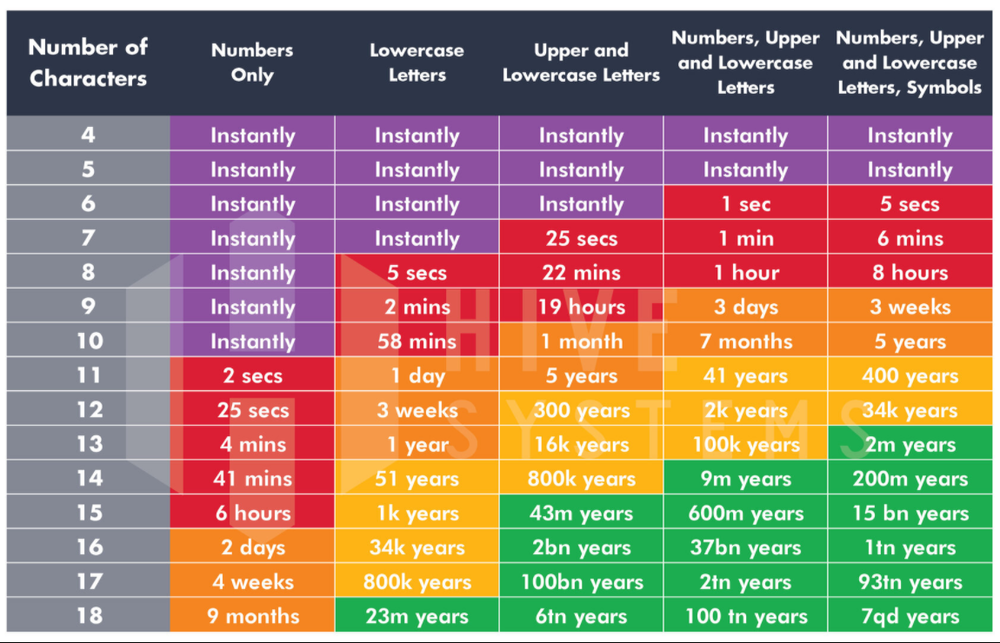
\includegraphics[scale=0.335]{./images/brute_force.png}
\captionof{figure}[Graph for secure passwords - The figure is taken from the homepage TechRepublic (https://www.techrepublic.com/article/how-an-8-character-password-could-be-cracked-in-less-than-an-hour)]{How secure is a password?}
\end{center}

Now if a user is not really sure if his or her password is secure, he or she can use a website like PasswordMonster to check how long it would take a hacker to crack his or her password.\cite{b9}


\subsection{Current state of art}
In recent years there was a massive increase in cybercrime. To prevent data-leaks, companies started integrating 2-factor-authentication.\cite{b4}\\
2-factor-authentication adds an extra layer of security to passwords. First the user has to key in the user name and password, which is the same as always. Then the user has to pass an additional login-method to verify it's really him/her.\\
The second factor is usually divided into these different types of categories:
\begin{itemize}
\item \textbf{Something the user knows.}  This might be a personal question the user had to configure beforehand, a personal identification number (PIN), etc.
\item \textbf{Something the user has.} This could be a small hardware token or smart-phone.
\item \textbf{Something unique to the user.} This might be a  biometric pattern like a fingerprint, an iris scan, or a voice print. 
\end{itemize}
The most common type of the 2-factor-authentication is a hardware token (Something the user has.). A leading company in this market is yubico. They are providing a security key named YubiKey for devices with USB-A, USB-C, Lightning and NFC. Users that have a YubiKey should be aware that they have to carry it with them at all time. If they lose it is unfortunate.\cite{11}\\
An other widely used method is the SMS Text-Message (Something the user knows.). After entering the password and user-name the user receives a unique one time passcode (OTP) via text message. They need to key in the passcode during a limited time (for example one minute). After both the first factor and second factor are correct the user gains access.

                                                                                               
\subsection{Future state of art}
In the future passwords will likely be replaced by passkeys because they are easier to use, securer, faster and work on almost every device.\\
A passkey is similar to the 2-factor-authentication but without the first factor. The second and only factor is the users device's security method such as a pin or a biometric sensor (fingerprint, face scan). \\
The passkey is hardware specific, which means the user always needs to carry the device (that the passkey is installed on) with them. If the user wants to use passkey on their laptop they need to verify their identity with their smartphone. This eliminates phishing, credential stuffing and other remote attacks. \\
In conclusion when a user is asked to sign-in to an app or website, he/she approves the sign-in with the same biometric or PIN that he/she uses to unlock the device (phone, computer or security key). The app or website can use this mechanism instead of the traditional (and insecure) username and password. \cite{b5}

\subsection{Solutions to password managing}
If users don't want to or can't use passkeys there are different options how they could protect their sensitive information. Users can write their passwords with account info into a booklet. The passwords would be unique and strong. It's a really simple idea but also has a lot of drawbacks. 
For example:
\begin{itemize}
\item Users need to carry the booklet with them everywhere. If not they can't always access their accounts.
\item Users can lose the booklet. If that happens they can't access any of their accounts any more.
\item It's not a really clear way of organizing passwords. Once something is written down user can't change the position in the booklet. So users would have to search for each password for indefinite time before they find it.
\end{itemize}
The other and better option is a password safe.  

\subsection{Password Safe}
\subsubsection{Explanation}
A password safe allows you to save a list of your user-names and passwords for all your accounts. It has one master password or passphrase that unlocks the safe. Now users only have to recall one single master passphrase instead of a huge amount of passwords.
\subsubsection{Examples}
\begin{itemize}
\item \textbf{KeepassXC}\cite{b6}\\ 
\begin{center}
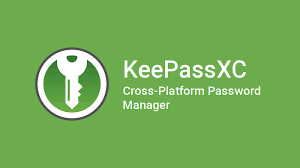
\includegraphics[scale=0.6]{./images/KeePass.png}
\captionof{figure}[KeePassXC - The figure is taken from the homepage of the KeePassXC Project (https://keepassxc.org/)]{KeePassXC Logo}
\end{center}

This software is developed for users with extremely high demands of secure personal data management. \\
KeePassXC uses Advanced Encryption Standard (AES) encryption algorithm with a 256-bit key to secure the password database.\\
The biggest difference to other password safes is that the data (password, account information and additional data such as URLs, attachments and notes) is stored in an offline, encrypted file that can be stored locally. This prevents user's data from getting leaked when a server gets hacked or breached.\\
The XC stands for Cross-Plattform. It is possible to use it on Linux, Windows, macOS and Android.\\
The program is customizable. It allows the user to customize literally everything to their needs.\\


\item \textbf{1Password}\cite{b7}\\
\begin{center}
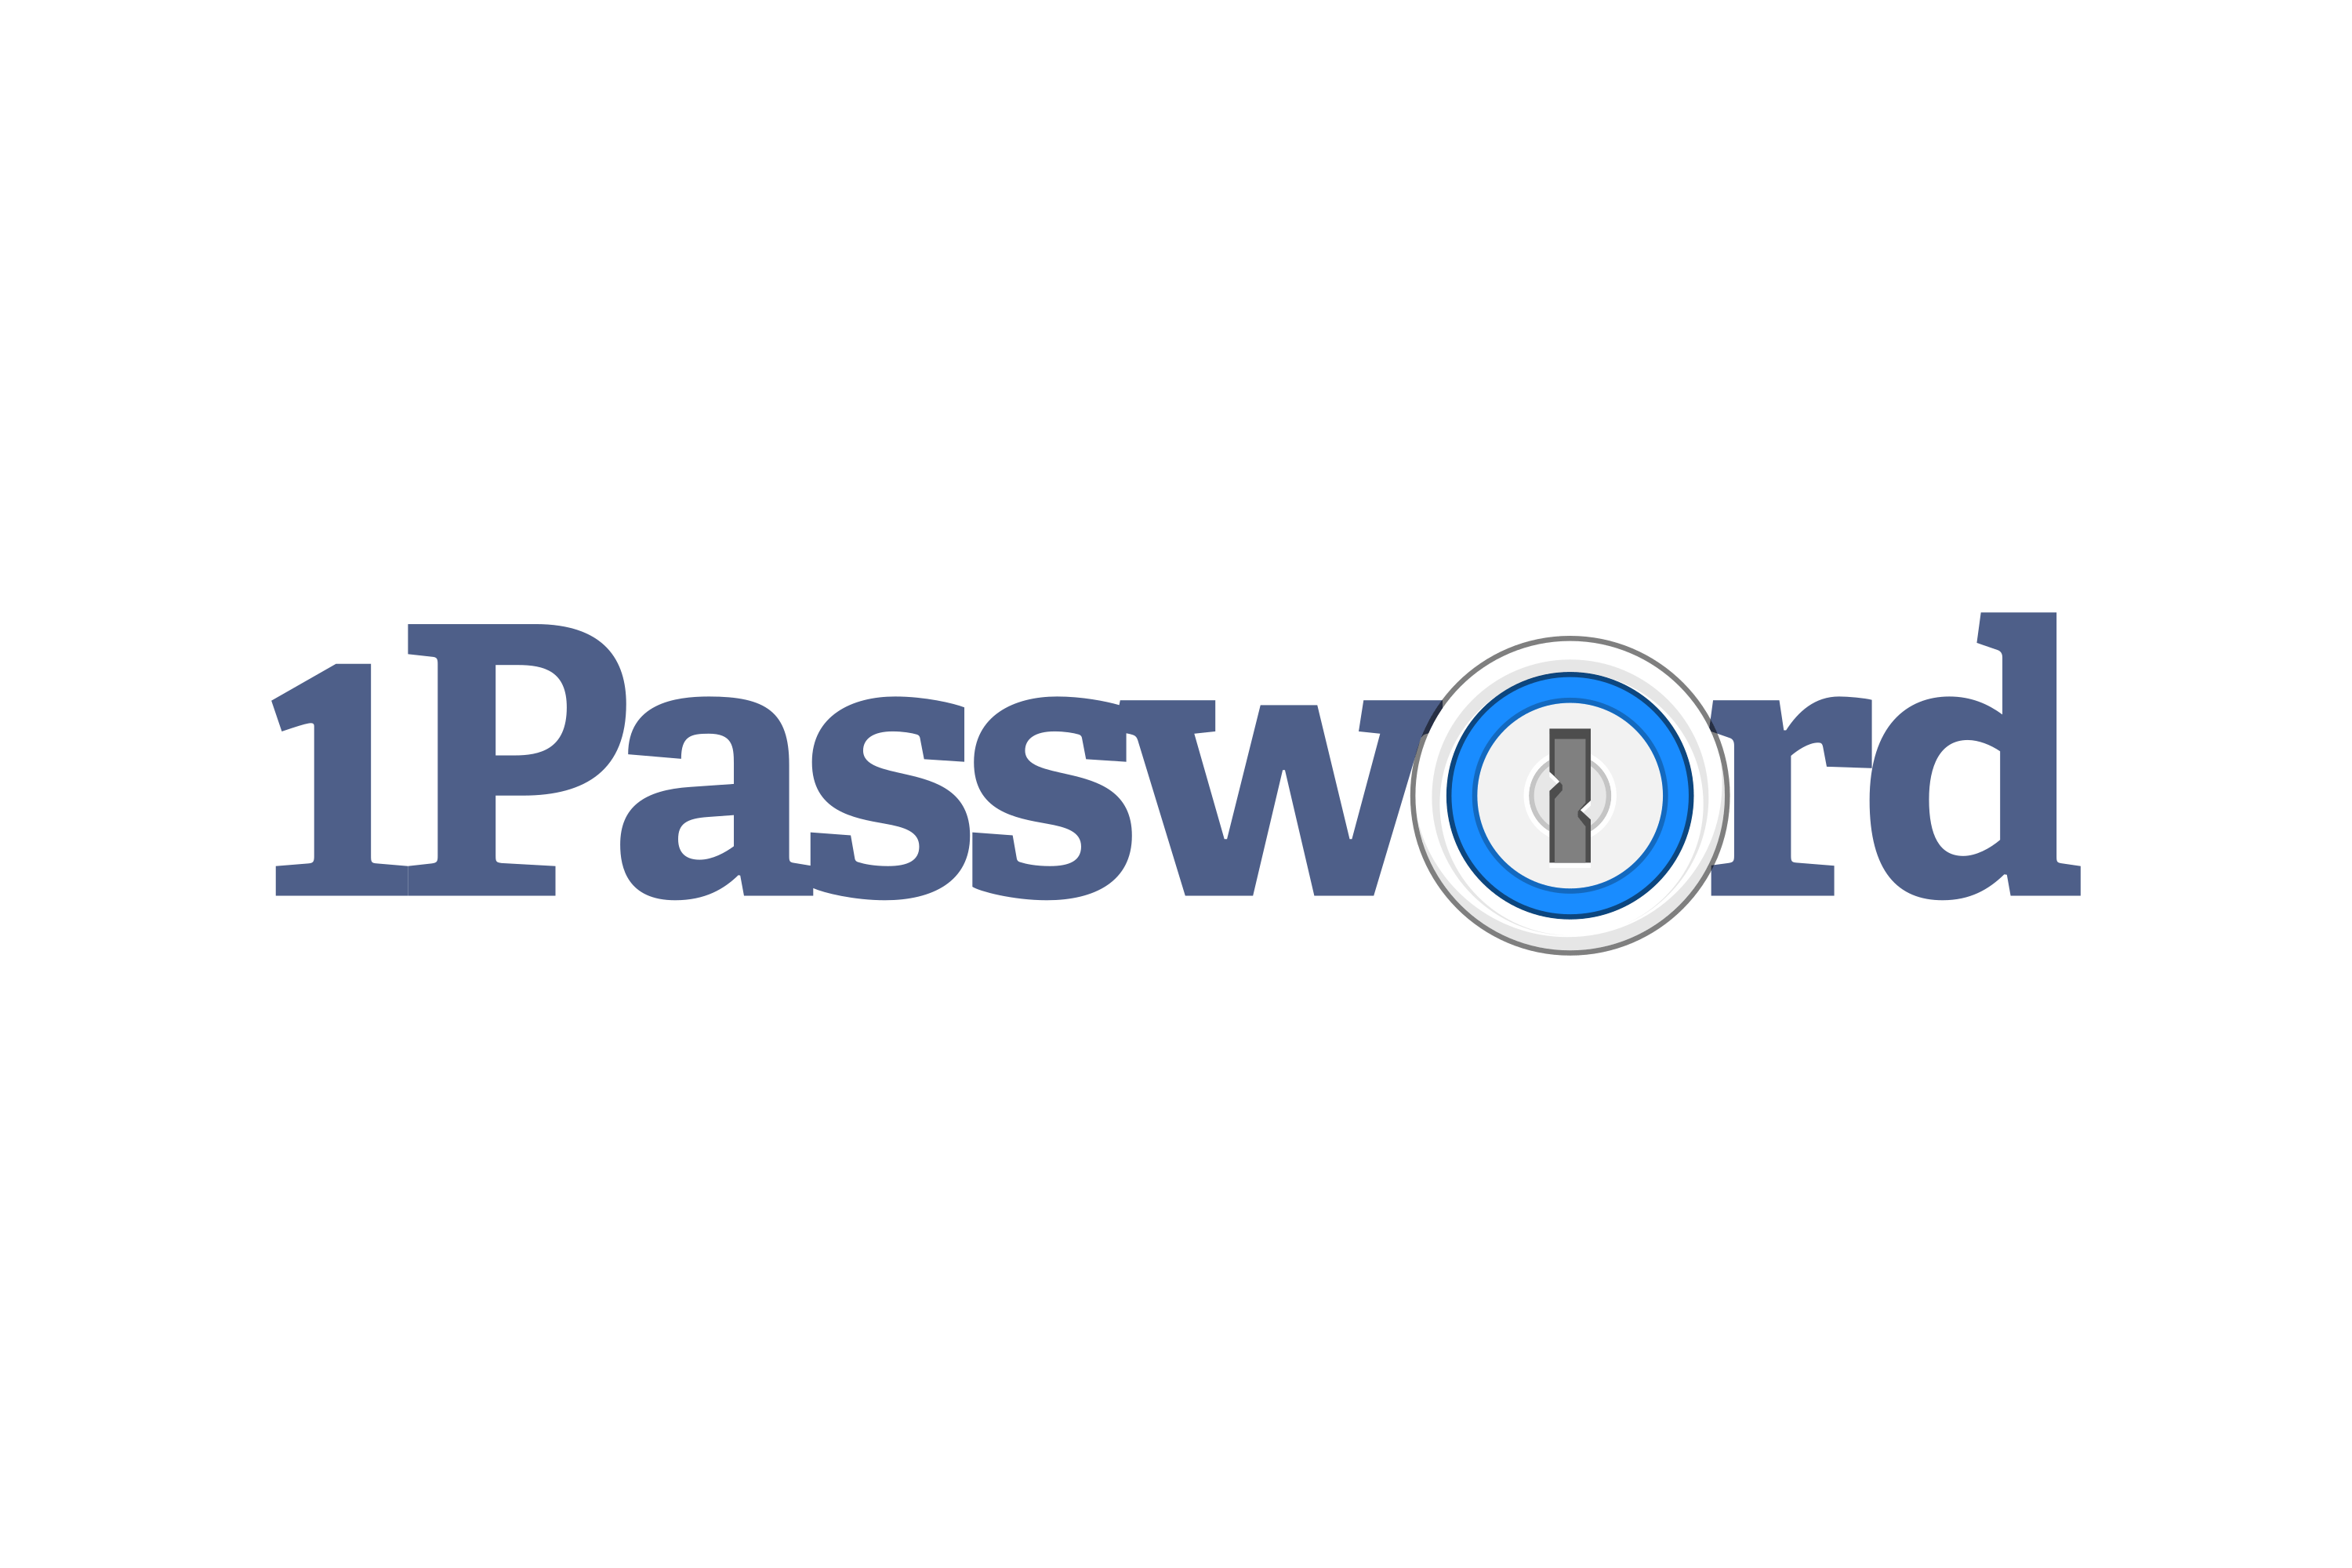
\includegraphics[scale=0.06]{./images/1Password-Logo.wine.png}
\captionof{figure}[1Password - The figure is taken from the homepage of the 1Password Project (https://1password.com/)]{1Password Logo}
\end{center}
This password safe is known for its easy to use interface and high security encryption.\\ 
1Password uses an uncommon encryption known as dual-key encryption. If the server gets breached it's impossible for the hacker to decrypt the user's sensitive information because of its two keys. The first key is the user's master-key. The second key is a secret key, which is a 128-bit, machine-generated code. The secret key is generated on every device the user logs into. It will only be saved on the user's devices and never saved together with the other pins.\\
Depending on what account type users choose their data is stored differently. However in only one version users have the option to save their data locally. In every other option the user's data gets saved in a cloud-based vault.\\
The interface is very user-friendly. It even generates strong passwords for accounts that are newly created.

    % Anwendungen (Methods): Verwendung, Welche System, Wie Gut, Ausmaß, https://www.usenix.org/system/files/sec22-mayer.
\end{itemize}
\subsubsection{Benefits and drawbacks of password safe software}\cite{b8}
\textbf{Benefits}:
\begin{itemize}
\item \textbf{Security:} Password safes use advanced encryption algorithms to protect the user's passwords. This makes it extremely difficult for hackers to steal the passwords and gain access to the user's online accounts.
\item \textbf{Convenience:} Password safes store all of the user's passwords in one place, which makes it easy for them to access their accounts without having to remember multiple passwords.
\item \textbf{Auto-fill feature:} Many password safes have an auto-fill feature that automatically enters the user-name and password for the user, saving them time and reducing the risk of typing errors.
\item \textbf{Multi-device access:} Many password safes allow user to access their passwords from multiple devices, including smartphones, tablets, and computers.
\item \textbf{Password strength:} Password safes often include a password generator feature, which creates strong passwords. This helps to ensure that the passwords are not easily guessable.
\end{itemize}
\textbf{Drawbacks}:
\begin{itemize}
\item \textbf{Single point of failure:} If a user's password safe is hacked or compromised, all of their passwords are at risk. It is important to choose a password safe that has a strong encryption algorithm and to use a strong master password.
\item \textbf{Dependency:} Using a password safe can make a user dependent on it for remembering passwords, which may make it difficult to remember passwords if a user is not able to access their password safe for some reason.
\item \textbf{Learning curve:} Some password safes have a steep learning curve, and it can take some time to get used to using them effectively.
\item \textbf{Cost:} Some password safes charge a fee for their services, which can be a disadvantage if user are looking for a free solution.
\item \textbf{Compatibility:} Some password safes may not be compatible with all websites or devices, which can limit their usefulness.
\end{itemize}



\section{Concept and implementation for best practise}
It can be very overwhelming to start with a secure option to manage passwords. So here is a best practise guide everyone can follow.
\begin{enumerate}
\item First you should check if your password has already been breached. There is a website that let's you easily check just that. It's called \textbf{"haveibeenpwned.com"}.\\
Haveibeenpwned is open source and secure. If someone searches for a breach it doesn't store the data that was typed in (an email address or phone number). It only ever retrieves the data from storage then returns it. \vspace{0.5cm}
\begin{center}
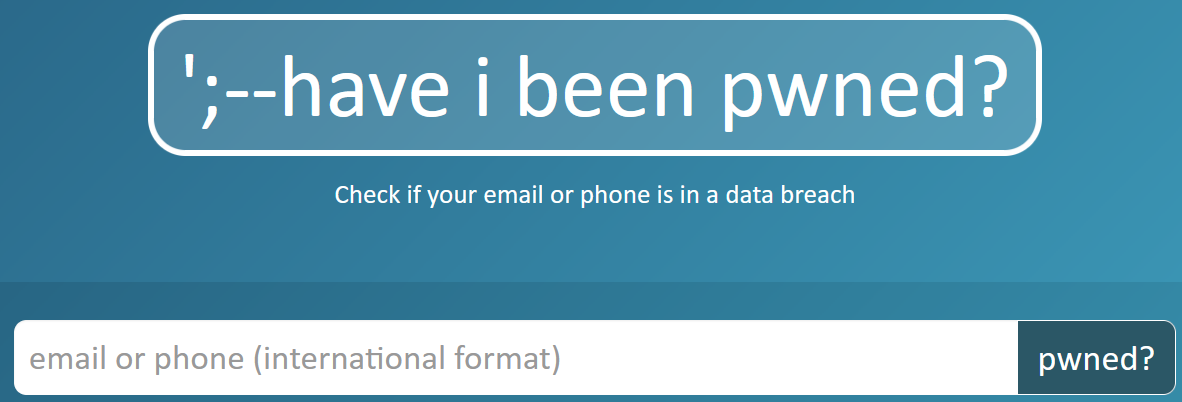
\includegraphics[scale=0.29]{./images/haveibeenpwned.png}
\captionof{figure}[Have I been pwned - The figure is taken from the homepage of the HaveIBeenPwned? Project (https://haveibeenpwned.com/)]{Have I been pwned? Homepage}
\end{center}
If you have already been pawned, change that password. If not you can rest assured. 
\item Pick a password safe that fits best for your needs. You can choose one of the ones mentioned above or do your own research.
\item Create a good master password or even better a master passphrase. Here is a easy way to do it: 
\begin{itemize}
\item First think of something which is easy to remember. For example "I love apples and bananas" or "Ich komme aus der Stadt Wien" if you want to use your native language.
\item The second step is to transform the sentence in dialect or slang form. For example "I luv appls and bananas" or "I komm aus da Stadt Wien".
\item Third, you can change letters into numbers and remove spaces. A "s" gets changes into a "5", an "e" gets changed into a "3" and an "o" gets changed into a "0". For example "Iluvappl5andbanana5" or "Ik0mmau5da5tadtWi3n".
\item The fourth step is to add symbols to your password. Change characters that look like a symbol into one such as "a" to "@" or "s" to "?". For example "Iluv@ppl5@ndb@n@n@5" or "Ikomm@u5d@5tadtWi3n".
\item The fifth step is to make all words start with a capital letter. This is only needed if the language you choose does not have a grammar rule for that (It's needed in English but not in German for example). 
\end{itemize}
In the end you would end up with a passphrase like "ILuv@ppl5@ndB@n@n@5" or "Ikomm@u5d@5tadtWi3n". This is a really secure passphrase because it has numbers, upper case and lower case letters, symbols and more that 8 characters. This would make a strong master password that is nearly impossible to crack.
\end{enumerate}


\section{Conclusion}
Passwords remain a widely used and convenient method of authentication, but they have significant weaknesses that make them vulnerable to attacks. While there are emerging alternatives to passwords, such as biometric authentication and passkeys, there are also challenges associated with their adoption, such as cost, compatibility, and user experience.\\
As the cybersecurity landscape continues to evolve, it is important to explore new, innovative and especially creative approaches to authentication and access control, that are both secure and user-friendly.


%Abbildungsverzeichnis erstellen
\listoffigures

\begin{thebibliography}{00}
\bibitem{b1} Proof for NordPass study, URL:https://tech.co/password-managers/how-many-passwords-average-person


\bibitem{b2} Information for "The problem with passwords", URL:https://www.nomios.com/news-blog/password-problem/ 

\bibitem{b3} List for most used passwords, URL:https://www.passwordmanager.com/most-common-passwords-latest-2022-statistics/

\bibitem{b4} Information for "Current state of art", URL:\\ https://authy.com/what-is-2fa/

\bibitem{b5} Information for "Future state of art", URL:\\https://fidoalliance.org/passkeys/\\ https://developer.apple.com/passkeys/\\ https://www.passkeys.io/\\ https://developers.google.com/identity/passkeys?hl=de

\bibitem{b6} KeepassXC, Open source password manager, URL: https://keepassXC.org

\bibitem{b7} 1Password, Paid password manager, URL: https://1password.com/de/

\bibitem{b8} Information for "Benefits and drawbacks of password safe software", URL: \\
https://expert.services/blog/managing-your-website/security/password-managers;\\ https://www.orangecountyscu.org/stories/pros-and-cons-of-using-a-password-manager/; \\ https://www.passwordboss.com/pros-and-cons-of-using-a-password-manager/; \\https://www.trustworthy.com/blog/pros-and-cons-password-manager/

\bibitem{b9} Link to PasswordMonster: https://www.passwordmonster.com/

\bibitem{b10} Resource for harmless example: https://www.heise.de/hintergrund/Roomba-Wie-private-Fotos-eines-Staubsauger-Roboters-auf-Facebook-landen-koennen-7457283.html

\bibitem{b11} Information for YubiKey: https://www.yubico.com/der-yubikey/?lang=de

\bibitem{b12} Resourece for Future examples: https://www.bostondynamics.com/

\end{thebibliography}

\end{document}
